\subsubsection{UC15.2.1 - Visualizzazione funzione del "list"}
\begin{figure}[h]
	\centering
	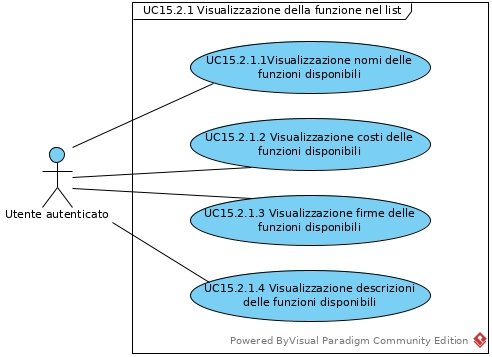
\includegraphics[width=0.7\linewidth]{res/img/UC15.2.1.jpg}
	\caption{Diagramma UC15.2.1 - Visualizzazione funzione del "list"}
\end{figure}
\begin{itemize}
	\item \textbf{Attori primari:} Utente autenticato;
	\item \textbf{Descrizione:} l'utente visualizzerà sul \textit{CLI\glo} i dettagli di una funzione del "list";
	\item \textbf{Pre-condizioni:} l'utente ha eseguito il comando "list";
	\item \textbf{Post-condizioni:} \textit{CLI\glo} visualizza le informazioni relative alla funzione presente nel sistema;
	\item \textbf{Scenario principale:} Il sistema mostrerà sulla \textit{CLI\glo} le informazioni relative a alla singola funzione visualizzata dal comando "list".
\end{itemize}
